Centralnym elementem, łączącym komponenty robota w całość jest drukowana płytka PCB (Printed Circuit Board). Jej ścieżki zastąpić miały dziesiątki kabli i przewodów łączących elementy. Proces budowy takiej płytki nie jest trudny i skomplikowany, pod warunkiem oczywiście, że człowiek wykona swoją pracę starannie, dokładnie i z pełnym oddaniem.

\subsubsection{Projektowanie}

Płytkę należało zaprojektować w odpowiednio dla tego celu stworzonym programie. Początkowo nasza płytka była tworzona w słynnym EAGLE'u, ostatecznie jednak porzuciliśmy go na rzecz KiCADa, ponieważ jest to narzędzie open-source, a takie oprogramowanie jest szczególnie bliskie naszemu sercu. Niestety, mimo naszej niechęci do zamkniętego oprogramowania nadal byliśmy zmuszeni skorzystać z systemu operacyjnego Windows.  

Projekt ten musiał być wykonany w odbiciu lustrzanym, tak, aby po odbiciu obrazu na płytkę, była ona w prawidłowym położeniu. Aby ułatwić sobie nieco sprawę, umieściliśmy na płytce napis „AKD’15 WI PP” ku chwale Akademii Kreatywnego Działania dr Rafała Klausa.
Prawidłowe odbicie takiego napisu na płytce wskaże, że wszystko poszło jak należy z zaprojektowaniem układu. 

Na wyjściu programu otrzymaliśmy jednostronną płytkę PCB. Niestety sieć połączeń nie zapewniała możliwości poprowadzenia naraz wszystkich połączeń bezkolizyjnie, dlatego też potrzebne było poprowadzenie paru połączeń dodatkowymi kablami. Dzięki temu udało się uniknąć konieczności projektowania znacznie bardziej skomplikowanej konstrukcyjnie płytki dwustronnej. 

\begin{figure}
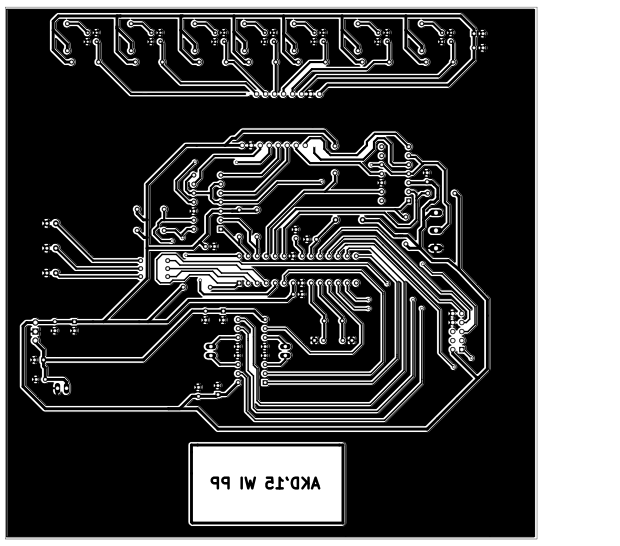
\includegraphics[scale=0.8]{board.png}
\caption{Płytka PCB naszego autorstwa}
\end{figure}
\subsubsection{Drukowanie}

Profesjonaliści biegli w konstruowaniu płytek dysponują sprzętem, który umożliwia konstruowanie płytek o wielu warstwach. Sprzętem takim dysponuje również nasza politechnika, lecz jak się okazało, korzystanie z podobnego sprzętu zostało zakazane. Zostaliśmy zobligowani do metody chałupniczej, tzw. żelazkowej, profesjonalnie nazywaną metodą termotransferową. Drukowanie postępowało w następujących etapach: 

\afterpage{%
\thispagestyle{empty}
\begin{figure}[!htbp]
\centering
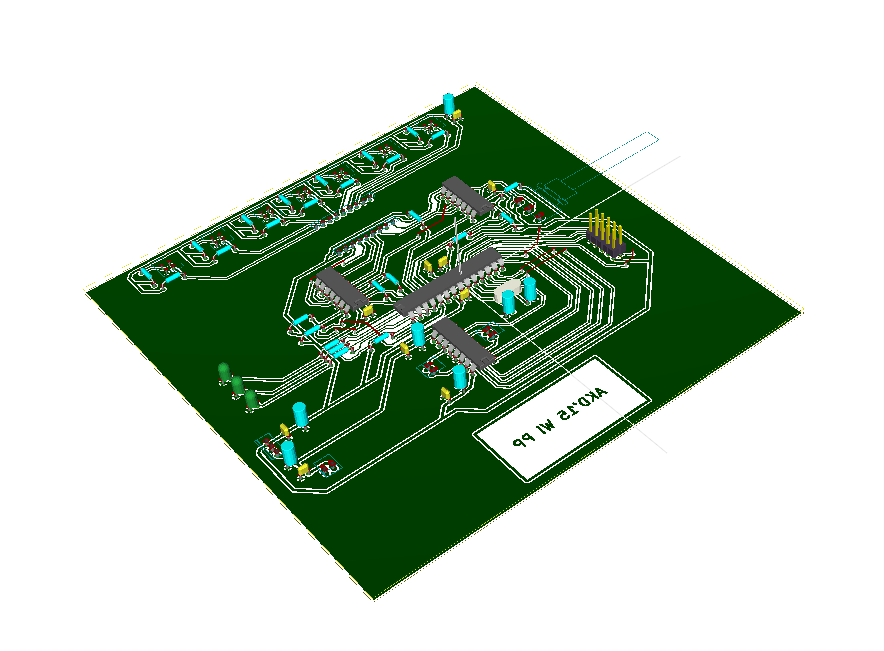
\includegraphics[scale=0.45]{gora.png}
\caption{Płytka PCB - rzut górny}
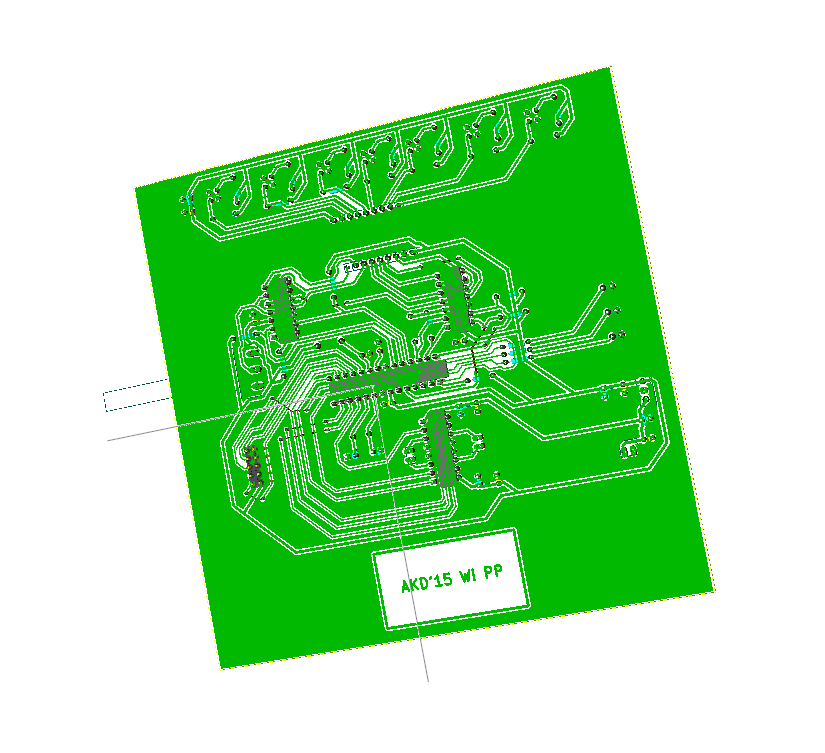
\includegraphics[scale=0.4]{dol.png}
\caption{Płytka PCB - rzut dolny}

\end{figure}
}

\begin{itemize}
\item Wydrukować drukarką laserową, w możliwie jak najlepszej jakości, obraz płytki powstałego w wyniku realizacji punktu 1. Preferowanym typem papieru jest tzw. papier kredowy, którego przewaga nad zwykłym papierem jest taka, że  jego powierzchnia jest bardzo śliska, dzięki czemu słabiej doń przywiera toner.
\item Następnie należy dociąć laminat do rozmiaru wydrukowanego obrazu. Jeśli nie jest on pierwszy raz drukowany, należy go bardzo dokładnie umyć z resztek toneru oraz innych zabrudzeń.
\item Przyłożyć papier kredowy do laminatu i dokładnie nałożyć papier, brzegi zaś kartki nie będące zadrukowane tonerem, użyć do przyklejenia do kartki. Zwrócić uwagę na fałdki papieru, brudy oraz inne podobne defekty.
\item Czwartym krokiem jest ogrzewanie płytki rozgrzanym żelazkiem. Ma ono być możliwie jak najcieplejsze. Dokładnie zgrzać całą powierzchnię kartki, zwracając również uwagę na brzegi kartki, zazwyczaj traktowane po macoszemu. Czas trwania kroku powinien wynosić ok. 15-20 minut. W wyniku okazać się ma, że cały toner został odklejony z papieru i odbił się na miedzianej stronie laminatu.
\item Po intensywnym działaniu termicznym na płytkę, włożyć ją do wody. Można dodać parę kropel detergentu. Płytkę trzymać w wodzie przez około 15 minut - dzięki temu papier zostanie dobrze odmoczony i będzie lepiej odchodzić od tonera. Po odmoczeniu płytki odkleić taśmę klejącą i zdjąć kartkę. Jeśli w wyniku tego nie odejdzie większa część obrazu, można przejść do kolejnego punktu, w przeciwnym razie należy powtórzyć całą procedurę powtórnie. Nasza grupa była zmuszona do trzykrotnego drukowania płytki na nowo. Nie należy zatem zrażać się niepowodzeniami, bo jest to klucz do sukcesu.
\item Następnie należy ostrożnie, z wyczuciem odpowiednim ścierać palcem resztki papieru - TYLKO W MIEJSCACH KTÓRE NIE SĄ POKRYTE CZARNYM TONEREM. Ułatwieniem jest z pewnością to, że białe miejsca nie są do niczego przyklejone, dzięki czemu teoretycznie łatwiej odchodzą. Należy co jakiś czas wkładać ponownie płytkę do wody, z powodu, że woda co jakiś czas znika z powierzchni płytki - głównie przez kontakt z dłońmi oraz w wyniku parowania. Należy uważnie odsłonić ścieżki, tak, że będą one błyszczeć miedzią, z której w rzeczywistości są zbudowane. Jest to najżmudniejsza część metody termotransferowej (nam zajęła około 2 godzin). Metoda ta jest przyczyną bólu rąk, dlatego też ważne jest by działać w zespole oraz wykazać się kreatywnością w konstrukcji narzędzi, np. małego rylca do zdzierania resztek papieru. Pomocą w takim wypadku jest Sz. P. Antonio Vivaldi, którego muzyka pomogła nam przejść ten uciążliwy proces. Serdecznie polecamy jego utwory młodym elektrotechnikom.
\end{itemize}

Przypadki obsługi niewielkich defektów płytki, takich jak zadarcia bądź niepełne odsłonienie ścieżek, zostało omówione w podpunkcie "Uwagi". Zalecamy jednak ostrożność w oczyszczaniu płytki.

\subsubsection{Trawienie}

Należy znaleźć odpowiednie naczynie, w którym umożliwiało zanurzenie w nim płytki w całości. Naczynie winno mieć odpowiednie parametry mechaniczno-chemiczne, takie jak: brak zewnętrznych otworów umożliwiające dyfuzję płynu trawiącego z otoczeniem (np. dziury) czy odporność na rozpuszczenie.

UNDER CONSTRUCTION

\subsubsection{Uwagi}

Często zdarza się, że palec producenta płytki jest zbyt szorstki, tak że zrywa większe połacie tonera, lub jego oko jest na tyle nie uważne, że nie dostrzegł że w którymś miejscu płytki ścieżka jest pokryta papierem. Nie  jest to powód do tego, aby ulec załamaniu nerwowemu oraz innym objawom głębokiej depresji.

W przypadku zdarcia czarnych elementów obrazu płytki, należy zaopatrzyć się w możliwie jak najcieńszy flamaster, o właściwościach zapewniających odporność na wodę. Właściwość ta daje ogromne szanse na to, że również ów tusz oprze się wytrawiaczowi. Należy wówczas dorysować zerwane części obrazu. W przypadku jednak, gdyby metoda ta nie pomogła, należy poprowadzić kabel zwykły między brakującymi ścieżkami. 

Innym defektem jest połączenie się ścieżek, w wyniku niedbałego ściągnięcia papieru z powierzchni płytki. Wówczas może dojść do zwarcia, czyli sytuacji, gdzie przewody nie stykają się w kontrolowany sposób, a raczej gdzieś pośrodku.  Należy problem ten rozwiązać poprzez przecięcie ścieżek nożem. Najlepszy zestaw do badania zwarć składa się z: diody, opornika 240 om, zasilania oraz dwóch przewodów. Należy szeregowo połączyć wszystkie elementy na płytce prototypowej. Przewody powinny być podłączone jednym końcem do obwodu, drugi zaś koniec powinien być wolny. Zetknięcie dwóch przewodów winno zamykać obwód i przyczynić się do zaświecenia diody - należy tak zbudowany zestaw obsłużyć. Jeden przewód powinien być przyłożony do masy, czyli do zewnętrznego obszaru płytki, nie mającego nic prócz miedzi, zaś drugim powinno się sprawdzać ścieżki układu, pilnując by nie zapaliła się dioda. W przypadku jej zapalenia łatwo wykazać, że doszło do zwarcia, i należy tą sytuację skorygować.